\chapter{Introduction}

%********************************** %First Section  **************************************
\section{Background and Motivation} 

\subsection{Company (Background)}
Würth Phoenix is a software company part of the Würth-Group specialized in the creation of ERP, CRM and IT System Management tools. The company is a certified Dynamics Gold Partner and works in close contact with Microsoft to develop and deploy state of the art solutions capable of meeting the clients requirements. The Dynamics AX department employs more than 70 certified consultants, system engineers and project managers specialized in the creation wholesale distribution software. One of the flagship products developed in this department in Trade+. Trade+ is a vertical solution based on Dynamics 365 (AX7) that offers additional functionalities built on top of the pre-existing Microsoft software that are specifically tailored to the needs of modern wholesale distributors. The application is the result of many years of experience in the field and comes from the long collaboration between Würth Phoenix and local and international companies that operate in the industry.

\subsection{Internship Project (Motivation)}
The latest iteration of the Microsoft Dynamics tool (D365) introduced a wide array of new features and represents one of the biggest evolution of this software in recent years. This shift in the industry standard makes it often difficult for developers to create reliable code that complies with the client needs while still maintaining an appropriate level of quality and reliability. Given the relative novelty of this update and the fact that the framework relies entirely on closed source code, finding good sources of documentation proves itself to be a particularly complex task. Most of the times (in the current stage of the tool lifecycle) said documentation does not exist and when it does is often particularly lackluster and fails to deliver any form of in-depth information. Because of this reason the motivation behind this project (and the work related to it) originates from the need of the company of having some form of practical know-how regarding the creation and implementation of test cases in a Dynamics 365 application.

%********************************** %Second Section  **************************************
\section{Objective} 

The goal of this project is to create a set of test cases covering some of the core functionalities of the application (Trade+) and integrating them with the nightly builds. A complementary objective is to document the process in order for the company to have some sort of guidance regarding schedules, complexity and resources needed to have (partial or total) test coverage. 
This includes not only the actual development process (i.e. coding) and all the activities related to it, but also procedures such as (but not limited to): identification of core processes, recording of high level tasks within the application, build integration, training, etc. Furthermore this work tries to present the difficulties encountered during the various stages of the process along with the approaches that had to be taken in order to overcome them. Particular attention is also placed in the comparison between the internal procedures previously implemented by the company and the (accepted, rejected or suspended) solutions proposed in this work.

%********************************** %Third Section  **************************************
\section{Initial approach}

We decided to organize the first phase of our work into two main activities that had to be carried out before establishing further details regarding the structure of the project. Said activities were:

\begin{itemize}
    \item Problem definition. A series of initial meetings were carried out in order to find a balance between the needs of the company and the overall skills required to complete the assigned work. Particularly important during this first phase was the definition of a "core" requirement that had to be initially given absolute priority and of some "secondary" tasks that could eventually be resolved once the main portion of the project was completed. During this stage a timetable containing both the project deadlines and the dates of the steering committees was also created. Said committees were periodical reunions organized to monitor the progress, review the content of the work, exchange feedback and adjust the scope of the project depending on the current situation.
    
    \item Training. Together with the previously described tasks an initial training period was planned in order to receive some basic knowledge regarding the covered topics, used technologies and company policies. Training activities were divided into face-to-face meetings and online lectures. The meetings covered an array of company-related subjects and were focused on the various functionalities of Trade+ (Wholesale and distribution, Retail, Production). The online lectures were provided by the Microsoft Dynamics Learning Portal and offered an in-depth analysis of the Dynamics 365 application, X++ programming language, Visual Studio development environment and TFS automation tool. Information where also provided regarding the differences between current (D365) and previous (AX) iteration of the Dynamics software.
\end{itemize}

Only when the company considered these activities covered to a sufficient extent to allow the execution of autonomous work was the attention gradually shifted to the first phases of the project.

%********************************** %Fourth Section  **************************************
\section{Method of work}

We decided to structure our work in the same way in which larger project are handled inside the company on a day to day basis. This meant basing the organization of the various stages of our work following the guidelines imposed by Microsoft SureStep.

\subsection{Microsoft SureStep}

Microsoft SureStep \cite{SureStepBook} is full life cycle methodology that helps partners develop, configure and implement Dynamics related solutions. The goal is to improve productivity and success rate while reducing costs and risk factors. This methodology also guarantees an higher degree of predictability during the implementation process and an increased involvement of the stakeholders. Furthermore both waterfall and iterative approaches guidelines are provided for delivering the solution. SureStep recognizes five distinct phases that can be interlinked in various ways in order to support different types of projects. Said phases are: 

\begin{itemize}
    \item Diagnostic. Activities related to the initialization of the project. An high level description and analysis of the customer process is formulated together with a first draft of the project plan where scope and approaches are initially defined. 
    \item Analysis. High level definition and documentation of the business processes are formulated together with the functional requirements. The training activities are also carried out during this phase.
    \item Design. Identification and planning of the implementation strategies and technical specifications together with data migration activities.
    \item Development. Implementation of new functionalities and adaptation of existing ones to satisfy the customer requirements. This phase also covers customer and acceptance testing. 
    \item Deployment. Setup of the functioning environment to the customer and system level testing. The deployment stage ends with the Go-Live.
    \item Operation. All activities related to a post Go-Live system (product support, project review, bug fixing, account management).
\end{itemize}

Another important activity of this methodology is the definition of team roles. Said role are divided between \textit{consulting} (project manager, business analyst, solution architect, application/development/technology consultant) and \textit{customer} (executive sponsor, purchase manager, IT manager, end/key user). SureStep provides a general definition of the tasks and skill required to cover each role. It is also necessary to notice that a person may cover multiple roles and that a single role can be assigned to multiple team members. 

\subsection{Structure}

Given the relatively small scope of the project described in this work we decided to apply the principles and phases of SureStep but to ignore certain specific activities that were typical of larger project and not applicable in this context. The Diagnostic phase started with the previously defined Kickoff meetings that allowed us to define a first version of the project plan with deadlines and objectives [Figure \ref{fig:projectPlan}]. The work environment was set up. During the Analysis phase we identified the test requirements of the application by analyzing its core features. The result of this phase was a definition of the required test cases. Said tests covered the following processes: Purchase order, transfer order, sales order, production order and return order. The training activities were also carried out during this phase. After this initial definition we started working (during the Design phase) directly on the application by utilizing an integrated tool, called task recorder, that allowed us to record high level (step-by-step) user interaction with the system. Said interactions were then converted into XML files that could be imported on any machine running Trade+ in order to reproduce the recorded process. At the end of this phase we had set of recordings covering the previously described features of the application. A built-in feature of the Visual Studio development environment allowed us to convert the task recordings into X++ coded test cases. This represented the starting point for the Development phase. Once created the test cases were expanded with tailored code specifically written to verify the expected behavior of the application under a wide array of different conditions and scenarios within the covered processes. The creation of test cases "ex novo" (not starting from a pre-existing recording) was also taken into consideration as a secondary requirement but later ignored given the level of expertise and knowledge of the system that such a task would have required. The last period of this phase was dedicated to the integration of the developed test in the CI workflow (i.e. nightly builds). In the context of this work the Deployment phase was reduced to a series of final meeting organized in order to communicate the project results and to hand in the documentation containing the experience know-how. All the further testing related work that will be performed on the application in the future will be part of the Operation phase.

\begin{figure}[ht]
	\centering
	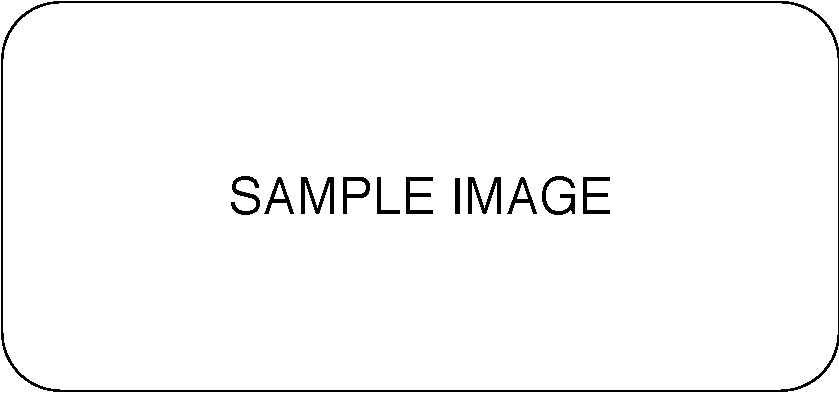
\includegraphics[scale=0.7]{Images/SampleImage.pdf}
	\caption{Project Plan}
	\label{fig:projectPlan}
\end{figure}